
%%%%%%%%%%%%%%%%%%%%%%
%                    %
% State of the Art   %
%                    %
\chapter{State of the Art}
\label{cp:soa}

In this chapter, we discuss the state of the art in energy modeling and optimization of computing hardware and mobile robots and in planning for mobile robots. There is a considerable body of knowledge in energy modeling for computing hardware, especially if battery-powered~\citep{rao2005battery}. When such hardware is onboard a mobile robot, studies on energy efficiency often focus on the energy for the motion on e.g., a planned path, and neglect the computing hardware~\citep{ondruska2015scheduled}. Moreover, planning algorithms in robotics literature center around robot motion planning and deal with problems such as swarms, dynamics, and uncertainty~\citep{lavalle2006planning}. By illustrating several contributions applied to a variety of robots, we primarily focus on the approaches that, similarly to ours, plans the path and schedules the computations. We especially emphasize studies applied to mobile robots with energy constraints.

We split the chapter into multiple sections and replicate our workflow throughout the topic. Initially, we analyzed some contributions that quantify the energy consumption of computing hardware carried by mobile robots. Modeling the energy of these devices has laid the foundations for our energy-aware planning. In~\fref{sec:soa-ene-mod}{Section}, we report our findings spanning broadly to generic computations energy modeling. We discuss the available approaches for battery modeling and the battery modeling and optimization of the mobile computing hardware in~\fref{sec:soa-ene-bat}{Section}. We then discuss studies on motion planning for mobile robots generically and planning for aerial robots in~\fref{sec:soa-motion-pl}{Sections}\fref{sec:soa-aerial-pl}{--\hspace{-.8ex}}. For both, we detail approaches in coverage path planning and the derivation of optimal coverage. Although simultaneous planning of computations and motion remains mostly unexplored~\citep{brateman2006energy,ondruska2015scheduled,sudhakar2020balancing}, some studies have proposed various techniques and further motivated our analysis. We report these in detail in~\fref{sec:soa-comp-motion-pl}{Section}.

This chapter connects to the remainder of this work as follows. Here we discuss the state of the art on topics that allowed us to derive a coverage planning and scheduling approach for autonomous aerial robots. Based on these findings, we later propose a computations energy modeling technique to derive
future energy consumption of mobile computing hardware along with motion in~\fref{cp:model}{Chapter}. Planning in the context of mobile robots, for aerial robots, of the coverage, and computations and motion, are the basis for the derivation of the optimal configuration in~\fref{cp:dyn}{Chapter}. We use such configuration to replan an initial plan; to solve the planning and coverage problems that we defined in~\fref{cp:pb}{Chapter}. \fref{cp:opt}{Chapter} then contains some further discussion of known principles in optimal control and state estimation that we extensively use in \fref{cp:dyn}{Chapter}.

%%%%%%%%%%%%%%%%%%%%%%%%%%%%%%%%%%%%%%
\section{Computations Energy Modeling}
\label{sec:soa-ene-mod}

There are several different energy modeling and optimization approaches for computations, usually under the topic of energy efficiency for computing hardware. Generally, energy efficiency is critical for battery-constrained devices~\citep{rao2005battery} and a limiting factor in improving further computing performance~\citep{horowitz2014computing}. 
Modern computing hardware--carried by aerial robots that we analyze in this work--is often composed of heterogeneous elements: one or more CPUs and a GPU as we outlined in \fref{sec:motivation}{Section}. We split some of the available approaches in the literature into different classes, depending on their modeling and optimization approach. Due to the unpredictable nature of the heterogeneous elements, many contributions to energy modeling observe hardware characteristics and perform physical energy consumption measurements to derive an energy model. We analyze some of these contributions first. They treat the heterogeneous elements altogether and are of particular interest to our approach where we use heterogeneous mobile computing hardware. We then analyze the techniques that focus on the energy of GPUs. Finally, we analyze techniques that treat CPUs. Some of the latter are based on dynamic voltage scaling (\Gls{acr:dvs})\findex{dynamic voltage scaling} and dynamic frequency scaling (\Gls{acr:dfs})\findex{dynamic frequency scaling} that scales down the supply voltage and the frequency when there is no high computations demand~\citep{flautner2001automatic, chen2009fundamentals}. Most of the studies we analyze include an energy model that is either an analytical expression (in the function of some architectural parameters of the computing hardware) or based on regression. The studies then provide an energy optimizing technique derived from the modeled energy. This latter is usually either the derivation of a selection of hardware parameters or a configuration of some computations parameters. We illustrate an overview of the studies we consider in \fref{tab:energy-models}{Table}, where we distinguish approaches by the heterogeneous elements, the model, and the technique they employ. We further state if a given study use DVS and/or DFS, summarize the accuracy, and report the experimental computing hardware when available (mobile and non).

There are some reviews available for computations energy modeling literature: O'Neal and Brisk~\citep{oneal2018predictive} summarize techniques with different computing elements and focus on predictive modeling emphasizing heterogeneous models based on machine learning. O'Brien~et~al.~\citep{obrien2017survey} and Czarnul~et~al.~\citep{czarnul2019energy} review energy modeling focusing on high-performance computing (HPC)\findex{high performance computing}; Czarnul~et~al. report existing tools for energy prediction in HPC systems and O'Brien~et~al. the accuracy of different models in the literature.

\begin{sidewaystable}
  \rotatesidewayslabel
    \footnotesize\fontfamily{phv}\selectfont
    \begin{tabularx}{\textwidth}{l|*{6}{l|}X|l}\hline
      &  & Model & Technique & Accuracy & DVS & DFS & Platform & Mobile \\
      \hline
      \multirow{8}*{\rotatebox{90}{Heterogeneous}} & Marowka & Analytical & Selection & - & \xmark & \xmark & Intel Core-i7-960 (CPU), NVIDIA GTX 280 (GPU) & \xmark \\
      & Bailey et al. & Regression & Configuration & 91\%\footnote{accuracy under-limit against oracle with perfect knowledge} & \xmark & \xmark & AMD A10-5800K (CPU), Radeon HD7660D (GPU) & \xmark\\
      & Goraczko et al. & Analytical & Configuration\footnote{optimization problem solved with ILP} & - & (\cmark) & (\cmark) & ARM7 OKI ML675003 (CPU), TI MSP430F1611 (microcontroller) & \cmark  \\
      & Ma et al. & - & Configuration & - & \cmark & \cmark & AMD Phenom II X2 (CPU), NVIDIA GeForce 8800 (GPU) & \xmark \\
      & Calore et al. & Analytical & Selection & - & \xmark & [\cmark] & ARM Cortex-A15 (CPU), NVIDIA GK20A (GPU) & \cmark\\
      & Yang et al. & Analytical & Pruning & - & \xmark & \xmark & - & \xmark\\\hline
      \multirow{5}*{\rotatebox{90}{GPU}} & Hong and Kim & Analytical & Selection & 91.06\%\footnote{average accuracy for both power and time models against measuring hardware} & \xmark & \xmark & NVIDIA GTX280 (GPU) & \xmark\\
      & Wu et al. & Regression (ML) & Selection & 90\%\footnote{\label{foot:avg-in-tab-energy-model}accuracy against built-in power monitors (if the accuracy is reported for multiple hardware or benchmarks, it is average)} & \xmark & [\cmark] & AMD Radeon HD 7970 (GPU) & \xmark\\
      & Collange et al. & - & Selection & - & \xmark & \xmark & NVIDIA G80, G92, GT200 (GPU) & \xmark\\
      & Luo and Suda & Analytical & - & 88.87\%\footnoteref{foot:avg-in-tab-energy-model} & \xmark & \xmark & NVIDIA Tesla C2050 (GPU) & \xmark \\
      & Leng et al. & Analytical & Selection & 88.35\%\footnoteref{foot:avg-in-tab-energy-model} & \cmark & \cmark & NVIDIA GTX 480, Quadro FX5600 (GPU) & \xmark \\\hline
      \multirow{6}*{\rotatebox{90}{CPU}} & Lee and Brooks & Regression & Selection & 95.7\%\footnote{accuracy against median error, leveraging only the most relevant samples} & \xmark & \xmark & - & \xmark \\
      & Takouna et al. & Regression & Selection & 93\%\footnote{accuracy of 95\% of the predictions} & \xmark & \cmark & Intel Xeon E5540 (CPU) & \xmark \\
      & Reddy et al. & Analytical & Selection & 94\%\footnote{accuracy on 60 workloads}\textsuperscript{, }\footnoteref{foot:avg-in-tab-energy-model} & \cmark & \cmark & ARM Cortex-A15 (CPU) & \cmark \\
      & Nikov et al. & Regression & Selection & 92--95\%\footnote{accuracy against related work} & \cmark & \cmark & ARM Cortex-A15, Cortex-A7 (CPU) & \cmark \\
      & Nunez-Yanez~and~Lore & Regression & Selection & 95\% & \xmark & \xmark & ARM Cortex-A9 (CPU) & \cmark \\
      & Walker et al. & Regression & Selection & 96.2--97.2\% & \cmark & \cmark & ARM Cortex-A15, Cortex-A7 (CPU) & \cmark \\\hline
    \end{tabularx}
    \caption[Comparison of different computations energy models]{Comparison of different computations energy models: the model is either an analytical expression or a regression. The energy optimization technique is the selection of some architectural parameters or computations configurations. Scaling is split into DVS and DFS: (\cmark) scaling is used only in the model, not in the optimization technique. [\cmark] values are changed statically (or manually where appropriate such as in Marowka).}
    \label{tab:energy-models}
\end{sidewaystable}

\subsection{Heterogeneous elements modeling}
\label{sec:soa-ene-hete}

Modern computing hardware energy modeling and optimization techniques often deal with the heterogeneous computing elements altogether using statistical tools. Such tools are inexpensive to deploy and relatively accurate in predicting the future energy consumption of computations~\citep{bailey2014adaptive}. Although there are further optimizations available by looking at the elements (CPUs, GPUs) separately, these are often application and hardware-dependent. Instead, we focus on a generic computations energy model that can be used independently of the hardware and computations under analysis. 

Marowka derives a model~\citep{marowka2017energy} for heterogeneous elements. The model uses some power metrics: the scaled speedup, scaled performance per watt, and scaled performance per joule. The approach increases energy efficiency by choosing the configuration of the heterogeneous components--for instance, by enabling computations only on CPU cores--and hence, investigates the impact of different architectural choices on energy efficiency. In particular, the model is used to analyze the energy of three processing schemes: symmetric, asymmetric, and simultaneous. The former uses merely a multicore CPU. Asymmetric processing scheme both CPU and GPU. The software benchmark on this scheme consists of running a program on one of the computing elements at a time. The latter processing scheme is similar to the previous, but the software benchmark runs on CPU and GPU simultaneously. Our work extends the model and builds a computations model to the simultaneous processing scheme.

Bailey~et~al. derive a more sophisticated statistical model~\citep{bailey2014adaptive} relying on multivariate linear regression for heterogeneous elements. The model eases the selection of the application's configuration that maximizes performance under given power constraints. It is trained offline with a small set of benchmarks and works across multiple devices. The overall flow of the proposed approach is composed of two stages. The first stage is the offline training stage that utilizes a small training set of benchmarks split into clusters. The model is built then with a regression per each cluster. After this stage, follows the online predicting stage. The latter uses the model to predict the power and performance of a large set of applications, opposed to the relatively small number of benchmarks in the offline stage. Our work similarly models a subset of samples and infers properties of the entire search space. Opposed to Bailey~et~al., our work further focuses on mobile computing hardware.

Goraczko~et~al. develop a resource model~\citep{goraczko2008energy} for heterogeneous mobile devices and consider both the time and power of a given run-time mode. Goraczko~et~al. use the term mode rather than configuration used by Marowka and Bailey~et~al. and use a CPU and a microcontroller\findex{microcontroller} as a heterogeneous platform instead of a CPU and a GPU. Energy-wise, the resource model uses DVS as some other models in \fref{sec:soa-cpu}{Section} but accounts for heterogeneous elements. The approach models multiple processors with a state machine involved in a software partitioning problem--the problem of deriving the optimal mode solved with an optimization technique: integer linear programming (ILP)\findex{integer linear programming}. The optimization occurs over an energy cost and with given deadline constraints. The intuition of formally defining the problem of deriving the optimal mode is similar in our work, expanded further by merging the path in our energy-aware planning and scheduling.

Ma~et~al. propose a holistic approach~\citep{ma2012holistic} for heterogeneous elements that achieves energy efficiency by splitting and distributing the workload among the heterogeneous elements. Ma~et~al. then use frequency scaling for the CPU and GPU and \Gls{acr:dvs} for the CPU. GPU-side, the frequency is determined with a lightweight machine learning algorithm. Energy in this approach is analyzed by empirical means, using two power meters. The testbed under analysis--NVIDIA GeForce GPUs and AMD Phenom II CPUs--does not include built-in power monitors, and overall, Ma~et~al. do not consider mobile computing heterogeneous hardware nor derive a model for the energy. Nevertheless, the approach is of interest for energy implications of heterogeneous elements.

Our initial approach~\citep{seewald2019hlpgpu} relied on external meters rather than internal power monitors. Calore~et~al. developed a similar technique~\citep{calore2015energy} to measure the energy efficiency of HPC systems. Both our initial and Calore~et~al.approaches are tested on the NVIDIA Jetson TK1 computing hardware that does not include built-in power monitors, opposed to other computing hardware that we analyze.

Recently, approaches are emerging to model the energy consumption of machine learning algorithms.
Yang~et~al. developed a computations-specific modeling approach~\citep{yang2017method} in this context, while Garc{\'i}a-Mart{\'i}n~et~al. surveyed several studies~\citep{garcia2019estimation}, motivated by the lack of appropriate tools to build and measure power models in existing machine learning suites. Garc{\'i}a-Mart{\'i}n~et~al. describe the state of the art of energy estimation for convolutional neural networks (\Gls{acr:cnn}s) and data mining\findex{data mining}, whereas Yang~et~al. evaluate an energy model of deep neural networks (\Gls{acr:dnn}s)\findex{deep neural network} based on a network bitwidth\findex{bitwidth}, sparsity, and architecture. The methodology applies exclusively to DNNs, but has been extended and used with CNNs~\citep{yang2017designing} in an optimization loop to reduce the computations energy consumption. Mittal then proposes a survey~\citep{mittal2019survey} to optimize and evaluate neural networks on some of the embedded platforms that we use in this work (NVIDIA Jetson TK1 and TX2). 

Kim~et~al. reviewed~\citep{kim2018survey} the operating system-level energy management techniques for heterogeneous elements. Although the review does not deal with energy models, it lists energy management techniques such as power-saving schedule that we utilize to dynamically optimize the energy resource of the aerial robots. They also detail aspects such as Quality of Service (QoS)\findex{quality of service} that we use to define execution boundaries for the computations.

\subsection{GPU features modeling}

GPUs are used in several applications despite increasing energy demands~\citep{mittal2014survey} due to their high computational resources~\citep{kasichayanula2012power}. It is hence unsurprising that for computations energy modeling, GPUs have their own modeling approaches. Here we discuss some studies of interest to our work. Mittal and Vetter and Bridges et al. propose extensive reviews of the available methodologies~\citep{bridges2016understanding,mittal2014survey}. Both are, however, not tailored to mobile computing hardware.

Hong~and~Kim derive an energy model~\citep{hong2010integrated} for GPU features. The contribution consists of an integrated power and performance prediction model to derive the optimal number of active cores for a given application to achieve energy savings~\citep{hong2010integrated}. The model is GPU specific: it consists of an analytical expression that estimates the GPU power and time in function of some parameters. Opposite to our work, it does not model the energy of the entire platform, nor is deployed on mobile computing hardware. Nevertheless, it achieves high accuracy in terms of GPU power and time prediction.

Wu~et~al. derive another model~\citep{wu2015gpgpu} with a similar focus on GPU features. The approach uses machine learning techniques for performance and estimates the power from real GPU hardware. In particular, Wu~et~al. train a neural network with different performance counters for various GPU configurations of a collection of applications and derive the optimal values of these counters. The approach works across multiple hardware; data gathered from one hardware estimates the power and performance of multiple other GPU hardware. However, Wu~et~al. focus purely on GPU modeling. Moreover, machine learning is an energy-expensive computation itself~\citep{garcia2019estimation,yang2017method}, thus deterring similar approaches in our planning, where we aim to preserve the energy as far as possible.

Collange~et~al. propose an empirical approach~\citep{collange2009power} for energy evaluations of GPUs during various computations in the CUDA\findex{CUDA} environment. The approach measures and analyzes how computations impact instantaneous energy consumption. It observes a significant energy impact of memory accesses and generally analyzes the energy cost of parallel GPU computations. The work by Collange~et~al. thus aims to derive the optimal memory configuration of a given benchmark. However, it does not use the measured data to calibrate a model for energy estimation nor focus on mobile computing devices.

Contrary to Collange~et~al.'s approach of pure empirical measurements, Luo~and~Suda\citep{luo2011performance} propose an analytical model for energy and performance estimation of GPUs. The model contains execution time and energy consumption prediction sub-models, where the latter follows from the former. The final analytical model for the energy estimation multiplies the execution time and the estimated power derived using an analytical expression. The work derives some observations on the energy implications of a given benchmark, which is then not used nor hypothesized in any energy adaptation technique. The accuracy analysis, redefined by the authors with another analytical expression, shows a strong correlation between observation and the analytical model. We also derive an analytical expression further motivated with empirical observation of energy data and employ a multivariate linear regression. We then focus on heterogeneous elements and mobile computing hardware.

Leng~et~al. propose a model~\citep{leng2013gpuwattch} based on a performance-per-watt metric for GPUs. Developed for general-purpose GPU (GPGPU)\findex{genral purpose GPU} powered devices, it is composed of multiple stages. An initial model is validated with some empirical measurements and eventually refined.  The contribution suggests an integrated power and performance modeling framework, which inputs a configuration to define micro-architectural and component parameters. It is then used in a feedback-driven optimization loop with the GPGPU. In our approach, we similarly input a configuration to the model, but we specify the computing hardware computations rather than architectural parameters. We use the output of the model in an optimization loop but extend this latter stage together with the path. Computation-wise, we use both heterogeneous elements.

\subsection{CPU features modeling}
\label{sec:soa-cpu}

Numerous other contributions model the CPU energy specifically and investigate how to lower the power~\citep{hong1999power, luo2001battery, chowdhury2005static} by some system-level optimization techniques. These include DVS, DFS, multiple asymmetric cores (such as the ARM big.LITTLE architecture), and power gating~\citep{walker2017accurate}. They usually incorporate information about configuration parameters into the scheduler~\citep{seewald2019coarse} and focus on homogeneous opposite to heterogeneous systems in our work. 

Lee~and~Brooks provide extensive coverage of regression modeling and propose a regression-based model~\citep{lee2006statistically,lee2006accurate} for microprocessors. The model uses a small number of samples of both the power and performance in a joint architecture-computations search space. The entire search space is sampled uniformly at random, an approach that allows identifying trends and trade-offs between the parameters~\citep{lee2006accurate}. The results show high accuracy even with a relatively small number of samples. We likewise use a regression model in our computations energy modeling approach but cover all the heterogeneous elements. Nonetheless, Lee~and~Brooks' approach is of interest to evaluate the accuracy of regression techniques and distributions of samples. Depending on the configuration space, we sample the computations uniformly using a linear or exponential distribution of samples (we specify the sampling distance in a configuration file), whereas Lee~and~Brooks sample architectural parameters.

Takouna~et~al. propose statistical multicore CPU\findex{multicore CPU} power models~\citep{takouna2011accurate} based on the average running frequency and the number of active cores. The models use multivariate linear regression commonly to other computations energy models in this section. Although insightful in terms of multicore CPU power models, the approach does not model GPUs nor heterogeneous elements and is tailored on virtualized serves, opposed to mobile computing hardware that we focus on in this work. Moreover, Takouna~et~al. do not consider computations configurations in the regression but a variable selection of architectural parameters.

Reddy~et~al. propose an empirical CPU power model~\citep{reddy2017empirical} that uses measured data and simulates the energy consumption of a quad-core ARM Cortex-A15 and gem5\findex{gem5}--a full-system architectural performance simulator. To collect the measurements, the model uses built-in power monitors in the ODROID-XU3 platform. Reddy~et~al. evaluate the model against sixty workloads reporting high accuracy on the ODROID-XU3 computing hardware. Our model shares compatibility with this computing hardware but is not simulator-dependent; we further evaluate the model on multiple heterogeneous computing hardware such as NVIDIA Jetson TK1, TX2, and Nano platforms.

Nunez-Yanez~and~Lore and Nikov~et~al. develop other models~\citep{nunez2013enabling,nikov2015evaluation} for mobile computing hardware. These models use hardware event registers and capture the state of the CPU under a representative workload. The latter study proposed by Nikov~et~al. is of particular insight, as they focus on ODROID-XU3 computing hardware; the model has three modeling stages: data collection of a benchmark running on the platform occurs in the first stage. The second and third stages are performed offline on a different architecture. They process the collected data (in the second stage) and generate the model (in the third stage)~\citep{seewald2019coarse}. The model further deals with ARM big.LITTLE architecture. We use these models to evaluate the performance of our computations energy modeling.

Walker~et~al. propose a run-time model~\citep{walker2017accurate} that uses performance monitoring counters (PMCs)\findex{performance monitoring counters} for mobile computing hardware, implemented on mobile CPUs such as ARM Cortex-A7 and Cortex-A15.  Walker~et~al. use the architectural performance simulator gem5 comparably to Reddy~et~al. and the ODROID-XU3 computing hardware to Nikov~et~al. The approach is to build a linear regression for a given CPU power prediction experiment. Although the study considers CPU-powered computing hardware only, it is insightful in terms of proposed statistical rigor in building run-time CPU power models.


%%%%%%%%%%%%%%%%%%%%%%%%%%
\section{Battery Modeling}
\label{sec:soa-ene-bat}

In this section, we describe some battery modeling approaches and focus on battery models that we can use with both the computing hardware and the aerial robot. There are several models for this purpose, each with its advantages and disadvantages.
Physical models use ordinary and partial differential equations to accurately predict the battery evolution in time~\citep{rao2003battery} but have a considerable time and computational cost~\citep{doyle1993modeling,marcicki2013design,lotfi2017reduced,moura2017battery}. Nevertheless, some hybrid models with less computational complexity have also emerged~\citep{kim2011hybrid,kim2019enhanced}.  Empirical models model the battery from a set of trials~\citep{syracuse1997statistical,pedram1999design} similarly to many computations energy models in~\fref{sec:soa-ene-mod}{Section}. They have a relatively low analytical insight~\citep{rao2003battery}, opposed to mixed models that derive some parameters from analytical expressions and experimental data~\citep{rao2003battery,rakhmatov2001analytical}. Abstract models use techniques such as the time evolution of an equivalent electrical circuit~\citep{gold1997pspice,benini2001discrete,seongjun2008state,xiaosong2012comparative,xing2014state,hasan2018exogenous} similarly to hybrid models~\citep{kim2011hybrid} but with less computational complexity. They have compelling trade-offs concerning analytical insight, accuracy, and complexity~\citep{rao2003battery} and are the models of our choice for battery modeling. Rao~et~al. survey~\citep{rao2003battery} the state of the art in battery modeling.

Xing~et~al. and Hasan~et~al. propose such abstract models~\citep{xing2014state,hasan2018exogenous} with an equivalent electrical circuit. These models model the battery state of charge (SoC) with the time evolution of a differential model of an equivalent circuit. The first model~\citep{xing2014state} utilizes an unscented Kalman filter\findex{unscented Kalman filter} to tune some parameters at each sampling step, and the second~\citep{hasan2018exogenous} estimates the SoC utilizing an eXogenous Kalman filter~\citep{johansen2017exogenous}\findex{eXogenous Kalman filter}. We use the model from Hasan~et~al. for the battery modeling. We derive an equivalent circuit for a Li-ion\findex{lithium ion battery} aerial robot battery and evaluate the SoC over time with a differential equation similar to the one proposed by Hasan et al.

Rao~et~al.~\citep{rao2005battery} propose a battery model for computing hardware specifically. The approach consists of an abstract stochastic model\findex{stochastic battery model} that uses Markov processes\findex{Markov processes} with probabilities related to the physical characteristics of the battery~\citep{panigrahi2001battery}. Rao~et~al. further improve the accuracy of the model, including some physical battery characteristics. The approach is insightful in terms of evaluating models for computing hardware. Indeed our approach relies similarly on an abstract model~\citep{hasan2018exogenous}, whereas we focus on an equivalent electrical circuit which requires less battery-specific knowledge for modeling. We can then model the SoC with little information regarding what battery the aerial robot mounts.

Zhang~et~al. propose a modeling technique for smartphones~\citep{zhang2010accurate} that consists of an automated modeling technique based on the battery discharge behavior and voltage sensors. The technique models the power using a multivariate regression (similarly to our approach and many computations energy models in \fref{sec:soa-ene-mod}{Section}) and the battery using an equivalent circuit. Although the analysis is limited to smartphones, it provides insights into automated modeling techniques for computing hardware. We have similarly derived an automated modeling technique for computations, battery, and entire system model in \fref{cp:model}{Chapter} that we integrate into our energy-aware coverage planning and scheduling.

Benini~et~al. propose a battery model~\citep{benini2001discrete} for the low-power design of computing hardware. The model, discrete-time and intended for system-level design environments, is also derived from an equivalent circuit. Although specific to the design of computing hardware applications, it evaluates different battery types: a first Li-ion implementation of the model is extended to various battery types with both non and rechargeable cells.


%%%%%%%%%%%%%%%%%%%%%%%%%
\section{Motion Planning}
\label{sec:soa-motion-pl}

Planning algorithms for mobile robots include broad and diverse topics. Energy-wise, the algorithms select an energy-optimized trajectory~\citep{mei2004energy}, e.g., by maximizing the operational time~\citep{wahab2015energy}. However, many studies apply to a limited number of robots~\citep{kim2005energy} and focus exclusively on planning the trajectory~\citep{kim2008minimum}, despite compelling evidence for the energy consumption also being significantly influenced by computations~\citep{ondruska2015scheduled,mei2005case}. 
In the remainder of this chapter, and before discussing the studies in mobile robotics that deal with computations and motion energy altogether, we detail planning in the literature. 
We are interested in planning and scheduling, and further recall that we are specifically interested in coverage planning of a given space in an energy-efficient way. We discuss the available literature on coverage planning for mobile robots later in this section and emphasize relevant studies for aerial robots in \fref{sec:cov-plan-aero}{Section}. There are multiple approaches in this sub-topic of motion planning~\citep{choset2001coverage,cabreira2019survey}, including studies that derive an energy-efficient cover~\citep{wei2018coverage,cabreira2018energy}. In \fref{sec:opti-cov}{Section} and \fref{sec:opti-aero-cov}{Section}, we discuss these studies respectively for mobile robots and aerial robots. 

Within simple motion planning instead of the derivation of a cover, Mei~et~al. propose an energy-efficient approach for mobile robots distinguishing the two energy consumers--the computations and motion energy. In~\citep{mei2004energy}, they focus on optimizing the motion energy and analyze the computations energy in a later iteration of their work~\citep{mei2005case}. We discuss the latter study in \fref{sec:soa-comp-motion-pl}{Section}. Their motion plan is composed of a path plan and a velocity schedule: the path plan is similar to ours in \fref{def:plan}{Definition}, and the velocity schedule contains velocities, accelerations, and decelerations along the route. Mei~et~al. then analyze the most energy-efficient path plan and velocity schedule; they evaluate the energy cost of a plan--of turns and accelerations--differentiating between the traveled against motors velocities. We have also optimized the coverage plan in \fref{sec:path-wise}{Section} compared to traditional coverage planning that uses, e.g., boustrophedon decomposition\findex{boustrophedon decomposition}~\citep{lavalle2006planning}. We do not consider a velocity schedule in our dynamic planning due to the physical constraints of airborne systems. Nevertheless, we also optimize the plan against sudden accelerations. Recall the plan in \fref{fig:plot3}{Figure} requires sudden decelerations in contrast to the plan in \fref{fig:plot4}{Figure} for fixed-wing crafts. Indeed one of the observations Mei~et~al. underline is the energy cost of turns. As an experimental setup, the study uses Palm Pilot Robot Kit with polyurethane omnidirectional wheels\findex{omnidirectional wheels} and three MS492MH DC servo motors. It relies on external power monitors to measure the power drain of the systems and five batteries: a 9 V battery and four 1.5 V batteries for the control circuit and motors. They measure the energy efficiency in terms of squared meters over jouls and report an improvement of 50\% by using an energy-optimized path plan. Mei~et~al. study has encouraged our initial analysis in energy-aware planning and scheduling in many respects. Mei~et~al. are the first study we found that analyzed motion and computations energy distinguishing explicitly for the need to account for computations energy~\citep{mei2005case}. However, Mei~et~al. lack further energy efficiency analysis in path variations. Indeed they focus on straight lines, spirals, and the energy cost of turns, whereas we focus on a generic variation in path within given limits. They do not explicitly address computations and motion planning yet propose foundations for future studies.

Dressler and Fuchs undertake a different approach to energy-efficient motion planning. In their work~\citep{dressler2005energy}, they focus on energy modeling of motion plans for given tasks (the term is not to be confused with computations), where, e.g., the mobile robot has to explore and supervise unknown surroundings. Dressler and Fuchs propose a future planning direction based on energy control and battery management for efficient tasks allocation but do not investigate further energy-aware planning. The study models energy-consuming parts of the robot with some corresponding characteristic curves. Dressler and Fuchs observe a linearly approximable curve for the SoC for some sub-tasks of a given task, such as movement and wireless communication. Although we do not model the energy of a given task, we similarly formulate the plan as a set of paths and computations in \fref{def:plan}{Definition} (of which we derive the optimal configuration energy-wise). The study has thus inadvertently introduced the differentiation between computations and motion energy that we have built upon. The reported sub-tasks energy models are indeed relative to one of the two components: wireless communication to a computation that
transfers data airborne, the movement to a path to reach the location. Dressler and Fuchs have further developed the approach, focusing on sensor networks~\citep{fuchs2006distributed,dressler2006lifetime}.

The majority of other contributions focus on optimizing motion planning to increase power efficiency. There are several studies that survey the available literature for mobile robots' planning, along with some textbooks~\citep{choset2005principles,lavalle2006planning}. Notably, La~Valle's textbook~\citep{lavalle2006planning} groups planning algorithms literature and focus on robot motion planning. Juli\'{a}~et~al. propose an extensive study of the most important methods for motion planning for autonomous exploration and mapping of unknown environments. The survey presents different techniques and classifies them for the level of multi-robot coordination and integration with simultaneous localization and mapping (SLAM)\findex{simultaneous localization and mapping} algorithm. 


\subsection{Coverage path planning}
\label{sec:soa-cov-path-plan}

In autonomous mobile robots scenarios, it is often required to explore every location in a given elemental region~\citep{cao1988region}; this latter problem is defined in the literature coverage path planning (CPP)\findex{coverage path planning} problem. In this section, we briefly discuss some surveys that deal with CPP in mobile robotics generically. We detail approaches that involve aerial robots in this latter sub-topic of motion planning in \fref{sec:cov-plan-aero}{Section}; in our work, we are dealing with this problem when we cover a given agricultural area in \fref{pb}{Problem}.
% I am the next par Adam. maybe move me in intro or pb?

CPP is related to the covering salesman problem\findex{covering salesman problem}, a variation of the famous traveling salesman problem (TSP)\findex{travelling salesman problem}: the salesman visits a neighborhood of each city, minimizing the travel length~\citep{arkin1994approximation}, and passes over all points rather than through all the neighborhoods~\citep{choset2001coverage}. This problem is sometimes referred to as the lawnmower problem~\citep{galceran2013survey} and is proven to be NP-hard~\citep{arkin2000approximation}. Early studies solve it using a heuristic with no coverage guarantee~\citep{choset2001coverage}. For instance, Arkin and Hassin propose simple heuristic-based algorithms for constructing the tours~\citep{arkin1994approximation}. There have emerged a variety of approaches ever since. Arkin appears in other studies that propose a continuous version for the covering salesman problem algorithm~\citep{arkin1993lawnmower,fekete1994lawnmower,arkin2000approximation}. These studies solve the problem with lawn moving and milling algorithms~\citep{arkin2000approximation}. Many approaches either implicitly or explicitly use cellular decomposition to guarantee the coverage (exact or approximate), decomposing the space to cover into cells; the overall solution to the coverage planning problem is then the union of the solutions of the cells~\citep{choset2001coverage}. 

To cover each cell in a cellular decomposition, the robot can use simple back and forth motion parallel to the cell's boundaries--often referred to as boustrophedon motion\findex{boustrophedon motion}~\citep{lavalle2006planning}--and reduce the coverage planning to motion planning between the cells~\citep{choset2001coverage}. The cells are geometric structures to represent the robots' free space and are decomposed into trapezoids in a popular class of solutions under the name of boustrophedon decomposition (since they are related to the boustrophedon motion). In this decomposition, the algorithm splits the origin cell in case of an obstacle (change in connectivity)~\citep{choset2000exact}. Choset~et~al. propose exact cellular decomposition method~\citep{choset1998coverage} that they complement with different motions in a later instance of their work~\citep{choset2000exact} (they consider, e.g., spiral, spike, diamond pattern, and others). Within the cellular decomposition method, some approaches~\citep{choset2000exact,acar2002morse} work with the concept of Morse function to indicate the location of cell boundaries. We show how does the boustrophedon decomposition proposed by Choset~et~al. work in \fref{sec:cell-deco}{Section}. Grid decomposition is another way of solving the coverage in the literature~\citep{zelinsky1993planning,gabriely2002spiral,shnaps2016online,wei2018coverage} that divides the space into equally sized cells. Other approaches are based on graphs~\citep{cheng2019graph} or derive an optimal coverage~\citep{huang2001optimal,xu2011optimal,lee2011smooth,li2011coverage,wei2018coverage}. The choice of the approach depends on the practical application~\citep{wei2018coverage}. The optimal coverage approaches are often a variation of known studies but with a cost that has to be optimized~\citep{galceran2013survey}. Our work fits into this latter class of approaches. In the remainder of this section, we discuss two surveys that deal with coverage planning and further detail relevant studies on optimal coverage. 

Choset proposes a survey~\citep{choset2001coverage} of literature on coverage for robotics. The survey classifies the studies according to the decomposition algorithm. The classification includes heuristic and cellular decomposition-based algorithms (approximate, partial-approximate, or exact cellular decomposition algorithms). Choset report that many algorithms for coverage planning with some guarantee in terms of either optimality or completeness are based on cellular decomposition. Approximate cellular decomposition algorithms described by Choset correspond to grid-based algorithms in other studies.

Galceran~and~Carreras propose one of such studies: a survey~\citep{galceran2013survey} of the different approaches for CPP. The survey classifies the algorithms among the others in online and offline classes, where the former rely on stationary information under a known environment and the latter on sensor measurements to sweep the space~\citep{galceran2013survey}. Like Choset, Galceran and Carreras report that most coverage planning algorithms decompose the space in sub-regions called cells to achieve coverage. The survey is extensive in terms of reviewed literature. It compromises studies focusing on cellular decomposition, cellular decomposition based on critical points of Morse functions\findex{Morse functions} (the latter can deal with generalized obstacles), graph (such as roads and streets networks), and grid algorithms. The work further surveys studies based on the detection of natural landmarks and approaches for robots with contact sensors. It covers methodologies operating in rectilinear environments, for 3D environments, for optimal coverage, for multiple robots, and based on reduction of the localization error.

\subsection{Optimal coverage}
\label{sec:opti-cov}

Huang analyzes an optimal coverage methodology based the cellular decomposition. The study~\citep{huang2001optimal} emphasizes the cost of performing turns and uses a boustrophedon-like motion that minimizes the number of turns. Huang utilizes round turns like the intuitive plan in \fref{fig:plot3}{Figure}. Huang minimizes the sum of sub-region altitudes--a metric related to the sweep direction of a sub-region. 
\begin{figure}[h]
  \centering
  \fontfamily{phv}\selectfont
  

\small
\def \globalscale {1.000000}
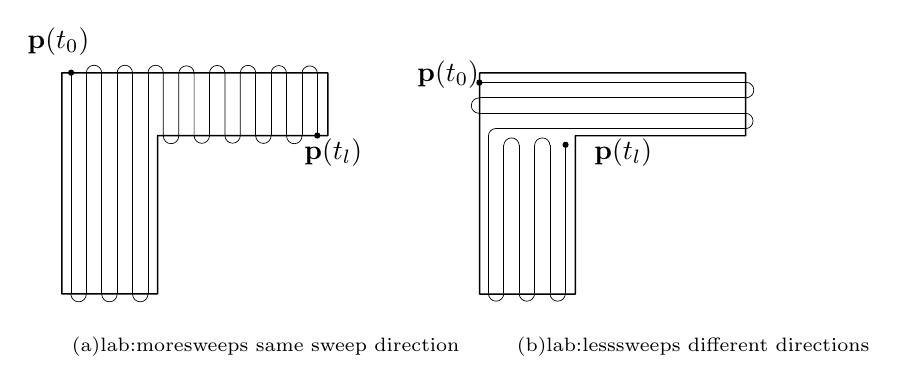
\begin{tikzpicture}[y=0.80pt, x=0.80pt, yscale=-\globalscale, xscale=\globalscale, inner sep=0pt, outer sep=0pt]
\path[draw=black,line join=round,line width=0.512pt] (15.4277,14.8977) -- (135.5920,14.8973) -- (135.5920,43.2656) -- (58.6591,43.2642) -- (58.6600,114.7730) -- (15.4277,114.7720) -- (15.4277,14.8977) -- cycle;



\path[draw=black,line join=round,line width=0.256pt] (19.5300,14.7961) -- (19.5300,114.8450);



\path[draw=black,line join=round,line width=0.256pt] (26.4900,114.8560) .. controls (26.4900,116.7780) and (24.9320,118.3360) .. (23.0100,118.3360) .. controls (21.0881,118.3360) and (19.5300,116.7780) .. (19.5300,114.8560);



\path[draw=black,line join=round,line width=0.256pt] (26.4900,14.7961) -- (26.4900,114.8450);



\path[draw=black,line join=round,line width=0.256pt] (26.4900,14.9536) .. controls (26.4900,13.0316) and (28.0481,11.4736) .. (29.9700,11.4736) .. controls (31.8919,11.4736) and (33.4500,13.0316) .. (33.4500,14.9536);



  \path[draw=black,line join=round,line width=0.256pt] (33.4561,14.7961) -- (33.4561,114.8450);



  \path[draw=black,line join=round,line width=0.256pt] (40.4161,114.8560) .. controls (40.4161,116.7780) and (38.8581,118.3360) .. (36.9362,118.3360) .. controls (35.0142,118.3360) and (33.4562,116.7780) .. (33.4562,114.8560);



  \path[draw=black,line join=round,line width=0.256pt] (40.4161,14.7961) -- (40.4161,114.8450);



  \path[draw=black,line join=round,line width=0.256pt] (40.4161,14.9532) .. controls (40.4161,13.0313) and (41.9742,11.4733) .. (43.8961,11.4733) .. controls (45.8181,11.4733) and (47.3761,13.0313) .. (47.3761,14.9532);



  \path[draw=black,line join=round,line width=0.256pt] (47.3661,14.7961) -- (47.3660,114.8450);



  \path[draw=black,line join=round,line width=0.256pt] (54.3260,114.8560) .. controls (54.3260,116.7780) and (52.7680,118.3360) .. (50.8460,118.3360) .. controls (48.9241,118.3360) and (47.3660,116.7780) .. (47.3660,114.8560);



  \path[draw=black,line join=round,line width=0.256pt] (54.3260,14.7961) -- (54.3260,114.8450);



  \path[draw=black,line join=round,line width=0.256pt] (54.3261,14.9531) .. controls (54.3261,13.0311) and (55.8842,11.4731) .. (57.8061,11.4731) .. controls (59.7280,11.4731) and (61.2861,13.0311) .. (61.2861,14.9531);



  \path[draw=black,line join=round,line width=0.256pt] (61.2793,15.0609) -- (61.2790,43.4113);



  \path[draw=black,line join=round,line width=0.256pt] (68.2392,43.4203) .. controls (68.2392,45.3423) and (66.6812,46.9003) .. (64.7592,46.9003) .. controls (62.8373,46.9003) and (61.2793,45.3423) .. (61.2793,43.4203);



  \path[draw=black,line join=round,line width=0.256pt] (68.2392,15.0609) -- (68.2390,43.4113);



  \path[draw=black,line join=round,line width=0.256pt] (68.2392,15.2181) .. controls (68.2392,13.2961) and (69.7973,11.7381) .. (71.7192,11.7381) .. controls (73.6411,11.7381) and (75.1992,13.2961) .. (75.1992,15.2181);



  \path[draw=black,line join=round,line width=0.256pt] (75.1759,14.8908) -- (75.1757,43.2412);



  \path[draw=black,line join=round,line width=0.256pt] (82.1358,43.2503) .. controls (82.1358,45.1722) and (80.5778,46.7303) .. (78.6559,46.7303) .. controls (76.7339,46.7303) and (75.1759,45.1722) .. (75.1759,43.2503);



  \path[draw=black,line join=round,line width=0.256pt] (82.1359,14.8908) -- (82.1356,43.2412);



  \path[draw=black,line join=round,line width=0.256pt] (82.1360,15.0480) .. controls (82.1360,13.1260) and (83.6940,11.5680) .. (85.6160,11.5680) .. controls (87.5379,11.5680) and (89.0959,13.1260) .. (89.0959,15.0480);



  \path[draw=black,line join=round,line width=0.256pt] (89.0892,14.8427) -- (89.0889,43.1931);



  \path[draw=black,line join=round,line width=0.256pt] (96.0491,43.2021) .. controls (96.0491,45.1241) and (94.4911,46.6821) .. (92.5692,46.6821) .. controls (90.6472,46.6821) and (89.0892,45.1241) .. (89.0892,43.2021);



  \path[draw=black,line join=round,line width=0.256pt] (96.0492,14.8427) -- (96.0489,43.1931);



  \path[draw=black,line join=round,line width=0.256pt] (96.0493,14.9996) .. controls (96.0493,13.0777) and (97.6073,11.5197) .. (99.5293,11.5197) .. controls (101.4510,11.5197) and (103.0090,13.0777) .. (103.0090,14.9996);



  \path[draw=black,line join=round,line width=0.256pt] (102.9940,14.9416) -- (102.9940,43.2920);



  \path[draw=black,line join=round,line width=0.256pt] (109.9540,43.3011) .. controls (109.9540,45.2230) and (108.3960,46.7811) .. (106.4740,46.7811) .. controls (104.5520,46.7811) and (102.9940,45.2230) .. (102.9940,43.3011);



  \path[draw=black,line join=round,line width=0.256pt] (109.9540,14.9416) -- (109.9540,43.2920);



  \path[draw=black,line join=round,line width=0.256pt] (109.9540,15.0983) .. controls (109.9540,13.1763) and (111.5120,11.6183) .. (113.4340,11.6183) .. controls (115.3560,11.6183) and (116.9140,13.1763) .. (116.9140,15.0983);



  \path[draw=black,line join=round,line width=0.256pt] (116.9410,15.0751) -- (116.9410,43.4255);



  \path[draw=black,line join=round,line width=0.256pt] (123.9010,43.4345) .. controls (123.9010,45.3564) and (122.3430,46.9145) .. (120.4210,46.9145) .. controls (118.4990,46.9145) and (116.9410,45.3564) .. (116.9410,43.4345);



  \path[draw=black,line join=round,line width=0.256pt] (123.9010,15.0751) -- (123.9010,43.4255);



  \path[draw=black,line join=round,line width=0.256pt] (123.9010,15.2318) .. controls (123.9010,13.3098) and (125.4590,11.7518) .. (127.3810,11.7518) .. controls (129.3030,11.7518) and (130.8610,13.3098) .. (130.8610,15.2318);



\path[draw=black,line join=round,line width=0.256pt] (130.8670,14.8597) -- (130.8670,43.2102);



\path[draw=black,line join=round,line width=0.512pt] (204.1270,14.9412) -- (324.2920,14.9408) -- (324.2920,43.3093) -- (247.3590,43.3079) -- (247.3600,114.8160) -- (204.1270,114.8150) -- (204.1270,14.9412) -- cycle;



  \path[draw=black,line join=round,line width=0.256pt] (324.4980,19.2296) -- (203.9500,19.2297);



  \path[draw=black,line join=round,line width=0.256pt] (324.4980,26.1896) -- (203.9500,26.1896);



  \path[draw=black,line join=round,line width=0.256pt] (324.3160,33.1874) -- (203.7680,33.1874);



  \path[draw=black,line join=round,line width=0.256pt] (324.1590,33.1476) .. controls (326.0810,33.1476) and (327.6390,34.7056) .. (327.6390,36.6276) .. controls (327.6390,38.5495) and (326.0810,40.1075) .. (324.1590,40.1075);



  \path[draw=black,line join=round,line width=0.256pt] (324.1290,40.0339) -- (211.5810,40.0339);



  \path[draw=black,line join=round,line width=0.256pt] (208.0900,43.5140) .. controls (208.0900,41.5921) and (209.6480,40.0341) .. (211.5700,40.0341);



  \path[draw=black,line join=round,line width=0.256pt] (208.0990,43.5067) -- (208.0990,114.5560);



  \path[draw=black,line join=round,line width=0.256pt] (215.0590,114.5660) .. controls (215.0590,116.4880) and (213.5010,118.0460) .. (211.5790,118.0460) .. controls (209.6570,118.0460) and (208.0990,116.4880) .. (208.0990,114.5660);



  \path[draw=black,line join=round,line width=0.256pt] (215.0590,47.6085) -- (215.0590,114.5560);



  \path[draw=black,line join=round,line width=0.256pt] (215.0590,47.7643) .. controls (215.0590,45.8423) and (216.6170,44.2843) .. (218.5390,44.2843) .. controls (220.4610,44.2843) and (222.0190,45.8423) .. (222.0190,47.7643);



  \path[draw=black,line join=round,line width=0.256pt] (222.0070,47.5074) -- (222.0070,114.5570);



  \path[draw=black,line join=round,line width=0.256pt] (228.9670,114.5660) .. controls (228.9670,116.4880) and (227.4090,118.0460) .. (225.4870,118.0460) .. controls (223.5650,118.0460) and (222.0070,116.4880) .. (222.0070,114.5660);



  \path[draw=black,line join=round,line width=0.256pt] (228.9670,47.6089) -- (228.9670,114.5570);



  \path[draw=black,line join=round,line width=0.256pt] (228.9670,47.7648) .. controls (228.9670,45.8428) and (230.5250,44.2848) .. (232.4470,44.2848) .. controls (234.3690,44.2848) and (235.9270,45.8428) .. (235.9270,47.7648);



  \path[draw=black,line join=round,line width=0.256pt] (235.9090,47.5074) -- (235.9090,114.5570);



  \path[draw=black,line join=round,line width=0.256pt] (242.8690,114.5660) .. controls (242.8690,116.4880) and (241.3110,118.0460) .. (239.3890,118.0460) .. controls (237.4670,118.0460) and (235.9090,116.4880) .. (235.9090,114.5660);



  \path[draw=black,line join=round,line width=0.256pt] (242.8690,47.6089) -- (242.8690,114.5570);



\path[draw=black,fill=black,line join=round,line width=0.512pt] (19.6152,13.7659) .. controls (20.2036,13.7659) and (20.6805,14.2429) .. (20.6805,14.8312) .. controls (20.6805,15.4195) and (20.2036,15.8964) .. (19.6152,15.8964) .. controls (19.0269,15.8964) and (18.5500,15.4195) .. (18.5500,14.8312) .. controls (18.5500,14.2429) and (19.0269,13.7659) .. (19.6152,13.7659) -- cycle;



\path[draw=black,fill=black,line join=round,line width=0.512pt] (130.8020,43.2046) ellipse (0.0301cm and 0.0301cm);



\path[draw=black,fill=black,line join=round,line width=0.512pt] (204.0410,18.2333) .. controls (204.6290,18.2333) and (205.1060,18.7102) .. (205.1060,19.2986) .. controls (205.1060,19.8868) and (204.6290,20.3638) .. (204.0410,20.3638) .. controls (203.4520,20.3638) and (202.9750,19.8868) .. (202.9750,19.2986) .. controls (202.9750,18.7102) and (203.4520,18.2333) .. (204.0410,18.2333) -- cycle;



\path[draw=black,line join=round,line width=0.256pt] (324.5100,19.2013) .. controls (326.4320,19.2013) and (327.9900,20.7593) .. (327.9900,22.6813) .. controls (327.9900,24.6032) and (326.4320,26.1613) .. (324.5100,26.1613);



\path[draw=black,line join=round,line width=0.256pt] (203.8550,33.1622) .. controls (201.9330,33.1622) and (200.3750,31.6040) .. (200.3750,29.6821) .. controls (200.3750,27.7601) and (201.9330,26.2023) .. (203.8550,26.2023);



\path[draw=black,fill=black,line join=round,line width=0.512pt] (242.9370,46.3286) .. controls (243.5260,46.3286) and (244.0020,46.8055) .. (244.0020,47.3939) .. controls (244.0020,47.9822) and (243.5260,48.4591) .. (242.9370,48.4591) .. controls (242.3490,48.4591) and (241.8720,47.9822) .. (241.8720,47.3939) .. controls (241.8720,46.8055) and (242.3490,46.3286) .. (242.9370,46.3286) -- cycle;



\path[cm={{1.0,0.0,0.0,1.0,(20.0,143.0)}}] (0.0000,0.0000) node[above right] () {\scriptsize \textlabel{(a)}{lab:moresweeps} same sweep direction};



\path[cm={{1.0,0.0,0.0,1.0,(221.0,143.0)}}] (0.0000,0.0000) node[above right] () {\scriptsize \textlabel{(b)}{lab:lesssweeps} different directions};



\path[cm={{1.0,0.0,0.0,1.0,(0.0,7.0)}}] (0.0000,0.0000) node[above right] () {$\mathbf{p}(t_0)$};



\path[cm={{1.0,0.0,0.0,1.0,(125.0,57.0)}}] (0.0000,0.0000) node[above right] () {$\mathbf{p}(t_l)$};



\path[cm={{1.0,0.0,0.0,1.0,(176.0,22.0)}}] (0.0000,0.0000) node[above right] () {$\mathbf{p}(t_0)$};



\path[cm={{1.0,0.0,0.0,1.0,(256.0,57.0)}}] (0.0000,0.0000) node[above right] () {$\mathbf{p}(t_l)$};




\end{tikzpicture}


  \caption[Turn optimal coverage with different sweep directions for each sub-region.]{An example~\citep{huang2001optimal} showing that different sweep directions for sub-regions in a cellular decomposition algorithm produce a coverage with an optimized number of turns; the robot moves from point $\mathbf{p}(t_0)$ to $\mathbf{p}(t_l)$ and in \sref{lab:lesssweeps} has almost half the turns of \sref{lab:moresweeps}.}
  \label{fig:huang}
\end{figure}
We illustrate the principle in \fref{fig:huang}{Figure}, where different sweeping directions produce a different number of turns. Huang proposes the methodology for both convex and non-convex shapes and uses dynamic programming for the optimal direction in the coverage. The approach performs better than other approaches by considering possible different sweep directions for different sub-regions. The study is insightful in terms of analyzing the coverage optimality of different directions in a boustrophedon-like motion. We similarly try to optimize the turns in our dynamic planning.

% While we will of- ten speak of the problem as "milling" with a "cutter," many of its important applications arise in various con- texts outside of machining. \citep{arkin2001optimal}
Arkin et al. have focused~\citep{arkin2001optimal,arkin2005optimal} on optimal coverage and have, similarly to Huang, considered the length of the tour with the number of turns. Both Arkin et al. and Huang remark that in many routing problems, the turns dominate the cost since the robot is often required to slow~\citep{arkin2001optimal}. Arkin et al.'s studies are insightful in terms of algorithmic rigor. They prove that coverage planning with turn costs is NP-complete even when the objective is merely to minimize the turns. To this end, they propose various approximation algorithms to compute nearly optimal covering tours. Nevertheless, the two studies and Huang's study are inconclusive in terms of nonholonomic robot constraints\findex{nonholonomic constraints}: they do not consider aspects such as the radius of the turn for optimal coverage. They also do not consider the eventuality of replanning in case external interferences affect the feasibility of the original plan. The latter scenario can happen in the eventuality of an aerial robot suffering a sudden battery drop while on a given optimal tour.
% We are obliged to Valentin Polishchuk for a very thoroughlist of suggestions, and thank three anonymous referees for various comments thathelped to improve the presentation of the paper.  We thank Regina Estkowski forhelpful discussions.

Shnaps and Rimon propose a solution to this latter problem and focus on robotics scenarios explicitly. In the study~\citep{shnaps2016online}, a robot has to cover an unknown environment with a strict battery constraint. Starting from a given point, the robot equipped with position and obstacles sensors navigates the environment and eventually covers the entire space. In a battery discharge event, the robot returns to the starting point to recharge the battery. Shnaps and Rimon model the energy cost with the path length and divide the space to cover into equally sized cells in a grid. Although insightful in terms of coverage planning for battery-powered robots, the approach does not account for aerial robots. Indeed in this latter class, the robots would require to land to recharge or replace the battery. Wei and Isler also consider the eventuality of strict energy constraints for mobile robots and revisit Shnaps and Rimon's approach. In the study~\citep{wei2018coverage}, they propose an algorithm restricted to axis-parallel motion generalized to arbitrary polygons. In both studies, the methodology is to divide the space into equally sized cells in a grid. The approach is tested on aerial robots, but is limited to rotary-wing crafts and generally unsuitable for nonholonomic robots' constraints. In both Shnaps and Rimons's and Wei and Isler's approaches, the energy optimality is considered within CPP rather than an integrated dynamic planning and scheduling approach in our work.

%%%%%%%%%%%%%%%%%%%%%%%%%%%%%%%%%%%%%%%%%%%%%%%%%%%%%%%%%%%%%
\section{Planning for Autonomous Aerial Robots}
\label{sec:soa-aerial-pl}

For what concerns planning for aerial robots, Popovi\'{c}~et~al. propose a study~\citep{popovic2017online} for planning and subsequent replanning to satisfy dynamic constraints. The study addresses the environment's disturbances and sensors' uncertainty using a noise-dependent model and accounts for a limited time budget. Popovi\'{c}~et~al. plan path online combining evolutionary optimization\findex{evolutionary optimization} and global viewpoint selection. They validate the approach with a precision agriculture scenario of detecting weeds. Although the proposed agricultural scenario has similarities with ours, it does not account for different aerial robots nor perform a dynamic energy replanning (of both the path and computations) in the function of battery state. Furthermore, the scenario does not require complete coverage, making it unsuitable for some applications we consider, such as hazard detection. Hayat~et~al. propose an approach~\citep{hayat2017multi} based similarly on evolutionary optimization in terms of multiple aerial robots planning of tasks and paths (the notion of task refers to a specific action rather than computation) for a search and rescue scenario. The approach has the same limitations as Popovi\'{c}~et~al.

Many other studies in planning for aerial robots under some energy constraints limit to energy-aware motion planning~\citep{wang2017curvature,morbidi2016minimum,kreciglowa2017energy}. They do not consider coverage planning nor disturbances. Kreciglowa et al. focus on the best trajectory between two hovering configurations in terms of energy efficiency~\citep{kreciglowa2017energy}. Morbidi et al. generate energy-optimal paths solving optimal control problems (\Gls{acr:ocp}s) to obtain the angular accelerations of four electrical motors of a quadrotor rotary-wing aerial robot~\citep{morbidi2016minimum}. 
%FROM THE BELOW STUDY; INTERESTING: There are two main categories of UAVs: fixed-wing aircraft and multi-rotor vehicles. Compared with multi-rotor vehicles, fixed-wing aircraft are more advanced in many respects: they tend to be more stable in the air in the face of both piloting and technical errors as they have natural gliding capabilities even without power, and they are able to travel longer distances on less power. More importantly, they have the advantages of being able to fly at high speeds for a long time using a simpler structure. These characteristics make fixed-wing vehicles still widely popular, despite requiring a runway or launcher for takeoff and being unable to hover. For these reasons, we consider the path planning problem for fixed-wing UAVs in this work.
Wang et al. propose a study~\citep{wang2017curvature}  of motion planning applied to the fixed-wing aerial robot. The approach passes through a set of waypoints by satisfying a given constraint on curvature.


\subsection{Aerial coverage path planning}
\label{sec:cov-plan-aero}

In the context of aerial robots, the survey~\citep{galceran2013survey} proposed Galceran~and~Carreras that we discussed in \fref{sec:soa-motion-pl}{Section} focus on optimal coverage~\citep{xu2011optimal} and multi-robot coverage~\citep{ahmadzadeh2008optimization,maza2007multiple,barrientos2011aerial,araujo2013multiple}. Our work come into the intersection of optimal coverage and coverage performed using aerial robots. Indeed in our coverage planning we dynamically refine a plan to achieve energy-aware behavior.

Cabreira~et~al. propose a survey~\citep{cabreira2019survey} that covers CPP exclusively for aerial robots. The study classifies the algorithms using the classification introduced by Choset~\citep{choset2001coverage} and Galceran and Carreras~\citep{galceran2013survey} from \fref{sec:soa-motion-pl}{Section} (the algorithms are split by cellular decompositions employed, and if they perform coverage online or offline). The survey further focuses on the shape of the coverage area and reports the performance metrics such as the path length, coverage time, and the number of turning maneuvers. Cabreira et al. focus on single and cooperative strategies for exact cellular decomposition and report the type of information used for the decomposition (full or partial). Remarkably, they analyze studies based on genetic algorithms\findex{genetic algorithm} and ant colony optimization\findex{ant colony optimization} and focus on different covering strategies and describe the so-called Zamboni motion\findex{Zamboni motion} similar to the fixed-wing plan in \fref{fig:plot4}{Figure}. 
Ara\'{u}jo~et~al. also analyze covering strategies~\citep{araujo2013multiple} for a given cell of interest. They describe the boustrophedon (that appears under the name ``lawnmower'')\findex{lawnmower} and Zamboni motion discussed in this work and additional spiral, spiral-like, Dubins path\findex{Dubins path motion}, modified boustrophedon\findex{modified boustrophedon motion}, and modified Zamboni motions\findex{modified Zamboni motion}.

While CPP under uncertainty for aerial robots appears in Cabreira~et~al.'s survey, there are two surveys~\citep{goerzen2010survey,dadkhah2012survey} with Mettler that review approaches dealing with uncertainty in general terms of aerial robots motion planning. The former survey~\citep{goerzen2010survey} emphasizes a classification based on differential constraints, grouping the motion planning algorithm with and without differential dynamics. The survey observes a lack in approaches dealing with uncertainty, whereas the latter~\citep{dadkhah2012survey} analyzes these explicitly. It groups the motion planning approaches by the class of uncertainty. For instance, in the case of uncertainty in vehicles' dynamics, the survey proposes studies based on optimal control and artificial intelligence. In the case of environment knowledge uncertainty, studies based on the mapping.

% In  a  survey  mission,  a  key  task  of  the  flight  planner  is  to  generate the UAV's path to completely cover the area of interest efficiently, and it is tackled with coverage path planning (CPP)
Nam~et~al. propose an approach~\citep{nam2016approach} for CPP for aerial robots that generates the covering tour offline. The approach uses a grid decomposition method, whereas the grids are visited using a wavefront algorithm\findex{wavefront algorithm}--a specialized version of Dijkstra algorithm\findex{Dijkstra algorithm} that optimizes the number of stages to reach the goal~\citep{lavalle2006planning}. Using the wavefront algorithm, they generate the optimal path between given points in space but do not focus further on optimal criteria. Indeed the practical analysis shows the result not being optimized with regards to the number of turns. Moreover, the approach focuses on rotary-wing aerial robots. Nam~et~al. do not deal with replanning in the eventuality of an unexpected event occurring nor account for energy explicitly, and the planning happens before the flight.

Sadat~et~al. propose an interesting approach~\citep{sadat2014recursive} for non uniformly shaped areas distributed into clusters, performing adaptive coverage depending on the distributions of the regions of interest in the space. Sadat~et~al. use coverage trees for the purpose (a structure where the child nodes cover the same area as the parents but with higher resolution) and propose different strategies to visit the tree (breadth-first\findex{breadth-first strategy}, depth-first\findex{depth-first strategy}, and shortcut heuristic\findex{shortcut heuristic}). Although insightful in defining the coverage area sparsely, the approach does not account for the aerial robot's battery nor discuss other aerial robots other than the rotary-wings.

\subsection{Optimal aerial coverage}
\label{sec:opti-aero-cov}

Di~Franco~and~Buttazzo propose an energy-aware CPP for aerial robots. The study~\citep{difranco2015energy} focuses on energy and other requirements, such as the completeness of the coverage and resolution. The energy model is generic for a given drone and outputs the energy consumption as a function of velocity and operating conditions using an interpolating curve of the power measurements. In particular, for future energy predictions, Di Franco and Buttazzo derive an energy model from measurements flying the drone in several conditions (during maximum acceleration and deceleration, horizontal flight, climbing, descending, hovering, and turns). The study hence proposes different analytical expressions derived from the interpolations for the scenarios. It covers a polygon with the boustrophedon decomposition similarly to \fref{fig:plot3}{Figure} but with sharp turns. Di Franco and Buttazzo then consider the quality of the coverage with varying distances between the coverage lines when the total modeled energy is lower than the available energy in an extension~\citep{difranco2016coverage} of the original study~\citep{difranco2015energy}. However, the latter study does not plan the coverage in flight nor focus on other aspects of the aerial robot. Furthermore, the energy model is plan specific--different paths have a different analytical expression for the future energy. Our model in \fref{sec:periodic-model}{Section} is generic, once trained with enough measurements for a given plan variation. The study is insightful for defining the energy cost of a given coverage and analyzes how variations in the coverage quality affect the power consumption. It uses an IRIS rotary-wing aerial robot\findex{IRIS rotary-wing aerial robot} (with four 850 Kv motors), a GoPro camera\findex{GoPro camera} mounted on a gimbal stabilizer\findex{gimbal}, and a PX4 flight controller. The systems are powered with a 3S 11 volts and 5.5 amperes per hour lithium polymer battery (LiPo) battery\findex{lithium polymer battery}. The aerial robot is not equipped with mobile computing hardware for computations, and the study does not consider other classes of aerial robots.

% VERY NICE STUDY
Concerning other related approaches for aerial CPP, Li~et~al. propose a study~\citep{li2011coverage} based on an enhanced cellular decomposition method. Li~et~al. plan the coverage in a polygon area and derive a covering methodology that minimizes the number of turns. The turns, already considered in the generic CPP by Arkin et al. and Huang~\citep{arkin2001optimal,arkin2005optimal,huang2001optimal}, are here further showed less efficient from energy, duration, and tour length points of view. For complex polygons, Li~et~al. propose a convex decomposition algorithm for minimum width sum based on the greedy recursive method. To connect the decomposed sub-regions, the authors propose a minimum traversal algorithm of a weighted undirected graph. The approach is complete in terms of algorithmic analysis. Li~et~al. provide the algorithms, analyze their complexity, and simulate the coverage on polygons of various shapes. They show their algorithms being optimal in terms of turns nonetheless, they do not consider further requirements for different aerial robots. Indeed a fixed-wing aerial robot has a greater turning radius compared to a rotary-wing aerial robot. Moreover, Li~et~al. plan the coverage offline. They do not consider unexpected occurrences derived from the robot's and environment's uncertainty, such as sudden battery discharge, wind gusts, and other atmospheric conditions; we take these aspects into account in our coverage planning. They further consider only path planning, opposed to planning the path along with the computations energy-wise while optimizing the battery usage.

% THIS IS a nice study that shows that turns are impractical when sharp with fixed-wings
Mannadiar~and~Rekleitis and Xu~et~al. propose studies~\citep{mannadiar2010optimal,xu2011optimal,xu2014efficient} on near-optimal complete coverage computed using a sequence of waypoints. The algorithms are near-optimal due to waypoint control having less maneuverability than velocity control~\citep{xu2014efficient}. They cannot thus guarantee optimality in terms of the tour length. The coverage algorithm~\citep{mannadiar2010optimal} was first presented by Mannadiar and Rekleitis and extended to non-holonomic robots~\citep{xu2011optimal,xu2014efficient} by Xu~et~al. The algorithm uses the cellular decomposition of a known environment with an arbitrary number of obstacles. The algorithm feds the decomposed cells into a Reeb graph\findex{Reeb graph}--an encoding used to compute a cyclic path where critical points are vertices and cells are edges~\citep{fomenko1997topological}. It then solves the Chinese postman problem\findex{Chinese postman problem}~\citep{eiselt2000historical} on the graph to derive the coverage order. The resulting path ensures that no cells are not traversed more than twice, with the robot returning to the starting point. Xu~et~al. analyze possible planning strategies for fixed-wing aerial robots and affirm that this latter class of robots lack the maneuverability needed to follow a sharp-turned path. Like Xu~et~al., we also generate paths that are to be followed by various classes of aerial robots, including fixed-wings. Xu~et~al. append a turning segment to the path by adding curlicue orbits at turns; whereas we incorporate the turning maneuver in our coverage planning rather than embedding external segments. Moreover, the studies do not focus on energy-aware coverage planning, on eventual replanning in case of adverse events, nor involve power-saving scheduling.

There are several other approaches for energy-aware aerial coverage. Cabreira~et~al. and Artemenko et al. propose studies~\citep{cabreira2018energy,artemenko2016energy} in this direction, focusing on photogrammetry in localization scenarios. Cabreira~et~al. propose spiral coverage for some polygon shapes and alter the velocity to achieve energy saving. Artemenko et al. propose a boustrophedon motion with smoothed turns using B\'{e}zier curves\findex{B\'{e}zier curves} but analyze other motions. However, Cabreira~et~al. and Artemenko et al.'s studies focus on a peculiar scenario rather than generic coverage. Another study provides an efficient coverage using different motion patterns for specific locations such as urban areas~\citep{dille2013efficient} but does not derive a generalized methodology. Some studies deal with optimal coverage deriving approaches~\citep{valente2013aerial,bouzid2017quadrotor} for rotary-wing aerial robots using interesting novel algorithms to find the optimal tour in a graph. In particular, Valente et al. use harmony search--a meta-heuristic algorithm based on musical harmony~\citep{geem2009music}--and Bouzid~et~al. use a genetic algorithm. Generally, all the studies in this paragraph focus on rotary-wing aerial robots. Although interesting in terms of analyzing the energy efficiency the studies do not propose replanning, nor power-saving scheduling.

%% optimal planning non aerial
%DONE 2 Optimal line-sweep-based decompositions for coverage algorithms
%DONE 7 Optimal covering tours with turn costs
%DONE 3 Coverage Path Planning Under the Energy Constraint


%% planning aerial robots

%%%% Zamboni these two were so so ...
%DONE 8 The ice rink problem
% proved zamboni is optimal is optimal to cover an area!
%DONE 5 !Path Smoothing! Paper with Khan et al.
% OUTCOME: Cite 1,19 when saying you cannot make sharp turn with a fixed-wing

%DONE 0 Online informative path planning for active classification using UAVs
%DONE -1 Multi-objective UAV path planning for search and rescue


%% aerial coverage
%DONE 15 An approach for coverage path planning for UAVs
%DONE 17 Recursive non-uniform coverage of unknown terrains for UAVs
%DONE 9 Curvature Continuous and Bounded Path Planning for Fixed-Wing UAVs 
%11 Multiple UAV area decomposition and coverage


%% optimal planning aerial
%DONE 4 Coverage path planning for UAVs based on enhanced exact cellular decomposition method


%DONE 1 Optimal complete terrain coverage using an Unmanned Aerial Vehicle
%DONE 19 Efficient complete coverage of a known arbitrary environmentwith applications to aerial operations
%DONE 18 Energy-Aware Spiral Coverage Path Planning for UAV Photogrammetric Applications
%DONE 13 Energy-Aware Trajectory Planning for the Localization of Mobile Devices Using an Unmanned Aerial Vehicle
%DONE 12 Efficient Aerial Coverage Search in Road Networks


%DONE 14 Quadrotor-UAV optimal coverage path planning in cluttered environment with a limited onboard energy
%DONE 16 Aerial coverage optimization in precision agriculture management: A musical harmony inspired approach


% okay this section, but we don't really contribute to any flight controller; so why to describe them...
%\subsection{\color{orange}Flight controllers}

%\subsection{\color{orange}Energy models in aerial robotics}

%\subsection{\color{orange}State estimation in aerial robotics}


\section{Planning Computations with Motion}
\label{sec:soa-comp-motion-pl}

Sudhakar et al. examine the trade-off between motion and computation energy for mobile robots in their recent study~\citep{sudhakar2020balancing}, focusing on robots with similar motion and computations energy. In the study, the robot moves on a path with a given length and velocity and, computations-wise, computes a specific number of nodes. Sudhakar et al. first derive an analytical expression for energy prediction that incorporates the path's length and velocity and the number of computations' nodes. The approach they propose consists of an algorithm for anytime planning\findex{anytime planning}--a planning approach that identifies an initial feasible plan then refined towards optimal over time~\citep{karaman2011anytime}. The algorithm eventually stops the refinements when it estimates computations energy exceeding the potential savings in terms of motion energy~\citep{sudhakar2020balancing}. To derive a path, the algorithm uses Bayes estimation\findex{Bayes estimation} on the edges of a graph in a sampling-based path planning algorithm--probabilistic roadmaps (PRM*)\findex{probabilitstic roadmaps} widely used in practice~\citep{lavalle2006planning,karaman2011sampling}. The study motivates our investigation and proposes an initial step towards further analysis. Nevertheless, it lacks rigor in deriving an energy model, and it does not account for battery SoC. Notably, Sudhakar et al. emphasize the importance of considering both the motion and computations for robots' energy-awareness; we share similar findings except for the study's claimed primate in analyzing trade-offs between motion and computations energy. By a closer inspection of the scientific literature, other studies have emerged in this direction. Mei~et~al., Sadrpour~et~al., and many others propose studies that deal with mobile robots motion and computations energy~\citep{mei2005case,mei2006deployment,brateman2006energy,zhang2007low,sadrpour2013experimental,sadrpour2013mission}. Recent contributions include work carried by Ondr\'{u}\v{s}ka~et~al. and Lahijanian~et~al.~\citep{ondruska2015scheduled,lahijanian2018resource}

Mei~et~al., which we already analyzed for their contribution to motion planning in \fref{sec:soa-motion-pl}{Section}, have proposed a study~\citep{mei2005case} analyzing both motion and computations energy. The study differentiates the microcontroller and embedded computer the mobile robot carries for a more flexible robot design. To this end, Mei et al. derive an energy model from empirical data and show that the motion accounts for less than 50\% of the total power consumption. Motivated by this finding on Pioneer 3DX ActivMedia\findex{Pioneer 3DX ActivMedia}--Pioneer mobile robots\findex{Pioneer mobile robots} from Adept MobileRobots\findex{Adept MobileRobots} were popular at the time of publication within the research community~\citep{erickson2003nonlearning,anguelov2004detecting,lemmay2004autonomous}--they propose real-time scheduling and dynamic power management to reduce the power consumption. The latter dynamically adjusts power states (e.g., DVS, DFS, and peripherals selection) of components without compromising overall performance~\citep{mei2005case}, and the former schedule computations energy-wise. The study is of particular interest as they quantify the computations' contribution to the overall energy expenditure of mobile robots. We further extend the study; it was indeed one of the starting points of our analysis. Yet, it does not implement the proposed techniques nor focus on planning within battery constraints--a research gap we are filling with our energy-aware coverage planning and scheduling. Mei et al. have extended their analysis in future instances~\citep{mei2006deployment,mei2005reducing,mei2005deployment} to CPP using multiple robots with both time and energy constraints. They have then solved repeated coverage~\citep{mei2006energy} but have not implemented computations scheduling nor focused on dynamic coverage replanning with sudden battery discharge. This latter aspect is of particular interest to aerial robots.

% good cite: Even though DVS and energy conservation for mobile robots have been studied, the close interaction between computation and motion remains unexplored
Brateman~et~al. propose an approach~\citep{brateman2006energy} on the intersection of modeling techniques for CPUs, which we discuss in \fref{sec:soa-cpu}{Section}, and planning computations and motion for mobile robots. The methodology varies the computing hardware's frequency and voltage via DFS and DVS and the motor's speed for energy efficiency. To find the best trajectory of the frequency, voltage, and speed over time, Brateman~et~al. formulate a nonlinear optimization problem (NLP) that they then solve using numerical optimization methods. The predicted energy is an analytical expression derived via probabilistic analysis that the methodology employs as an optimization cost within a time constraint. There are many more approaches that employ optimization techniques for energy-efficiency of computations and motion in mobile robotics~\citep{zhang2007low,ondruska2015scheduled,lahijanian2018resource}. Zhang~et~al. vary the robot's speed and the computing hardware's frequency using optimal control on a random horizon. To this end, they transform an optimal control problem (OCP) into a nonlinear optimization problem (NLP) and solve the latter using a standard numerical optimization approach. The OCP has an analytical expression of the frequency and speed as the cost~\citep{zhang2007low}. Interestingly, they also derived an analytical solution to the OCP for some simplified costs and found up to 30\% energy savings compared to the heuristics methods. Like Brateman et al. and Zhang et al., we derive an OCP for replanning the coverage in \fref{cp:opt}{Chapter} but vary the coverage path and the schedule on the computing hardware rather than the frequency, voltage, and speed. The intuition behind our more complex planning is that by scheduling and replanning appropriately, we can ensure coverage despite external adversities.

Sadrpour~et~al. focus on mission energy prediction--the energy needed to complete a given set of tasks by the robot traveling some paths while interacting with the environment~\citep{sadrpour2013mission}--for unmanned ground vehicles (\Gls{acr:ugv}s)\findex{unmanned ground vehicle}. In their two studies~\citep{sadrpour2013mission,sadrpour2013experimental}, Sadrpour~et~al. propose two prediction approaches depending on a priori mission knowledge (i.e., constant power drain of static components, driving style, road rolling resistance, road grade information, and vehicle internal resistance). In case of no a priori knowledge, they propose linear regression and Bayesian estimation otherwise. Sadrpour et al. report the findings on the energy prediction using PackBot UGV\findex{PackBot UGV}~\citep{yamaichi2004packbot}: the computations have an order of magnitude lower consumption than motion. Notably, Sadrpour and other researchers shared some findings in later studies~\citep{sadrpour2014real,ersal2014keeping} in the direction of UGVs performing CPP. Although the studies and their later iterations focus on energy modeling, they propose a future instance in dynamic mission decision-making. When the energy exceeds a reasonable threshold, the UGV might, e.g., revise the initial plan or tune energy-expensive components~\citep{sadrpour2013mission}. Our dynamic planning shares a similar principle of tuning the plan to accommodate energy expenditure. We further focus on computational aspects, as in the mobile robots under our study--and nonetheless, in recent energy-efficient robotics platforms--the motion energy has the same order of magnitude as computational energy~\citep{sudhakar2020balancing}.

% Robots require energy to operate. Yet they only have access to limited energy storage during missions.
% good references for planetary exploration rovers, indeed ARC Q14 is implemented for this latter purpose
%  the energy  budget  for  sensing  and  computing  is  commensurate with  that  of  actuation  -  such  as  is  typically  the  case  forplanetary rover missions.
More recently, Ondr\'{u}\v{s}ka~et~al. proposed a study~\citep{ondruska2015scheduled} to reduce energy consumption by scheduling navigation at given times while traveling a path. The study focuses on Oxford Robotics Institute\findex{Oxford Robotics Insitute} (ORI) ARC Q14\findex{ARC Q14} mobile ground-based robot--a robotic platform used mainly for research in planetary exploration rovers~\citep{yeomans2017murfi}--following a predetermined path and accounts directly for computations energy. Ondr\'{u}\v{s}ka~et~al. propose to schedule the navigation so that the robot remains within a margin from a given path. For the scheduling itself, Ondr\'{u}\v{s}ka~et~al. derive two algorithms. A greedy algorithm guarantees feasibility by employing a simple heuristic, and a belief planning algorithm uses optimal control to provide energy-efficient schedules on a given horizon. The approach considers path following rather than CPP, yet it is of interest in many respects. Firstly, Ondr\'{u}\v{s}ka~et~al.'s algorithm is based on optimal control. It is similar to ours based on output model predictive control (\Gls{acr:mpc}). Secondly, the algorithm runs on a finite horizon. We employ the same technique for replanning. Finally, the approach further motivates our planning: Ondr\'{u}\v{s}ka~et~al. report a saving of 11.5\% using a power-saving scheduler on the robot. Our methodology alters both the schedule and the path for aerial CPP.

% good cite: 
Lahijanian~et~al. have further extended Ondr\'{u}\v{s}ka~et~al.'s work and proposed a framework~\citep{lahijanian2018resource} for resource-performance trade-offs exploration. They find a schedule for mobile robots under a given resource budget using quantitative multi-objective verification and controller synthesis\findex{multi-objective verification and controller synthesis}--a technique that starting from constraints, such as time and energy, produces a set of optimal achievable trade-offs via Pareto front\findex{Pareto front}~\citep{forejt2012pareto}. Although insightful in selecting the best schedule, the approach does not account for dynamic planning, whereas in our work, an initial plan accounts for the highest achievable performance. These are then replanned both path- and computations-wise in an energy-aware fashion. Lahijanian et al. also use the ARC Q14 robot.

\section{\color{red}Summary}

